%-  LaTeX source file

%-  section3.tex ~~
%
%   This is the third section of the paper.
%
%                                                   ~~ last updated 27 Nov 2018

%\begin{itemize}
%    \item Start of project and proof of concept, restrictions caused by policy
%        of usage of OLCF
%    \item Adaptation of already existed PanDA application to work with Titan
%    \item Many To One concept (Many jobs - one pilot)
%    \item First implementation (Multijob Pilot as evolution of PanDA Pilot)
%    \item Scalability limitations
%    \item Harvester
%\end{itemize}

Consistent with its leadership-computing mission of enabling applications of
size and complexity that cannot be readily performed using smaller facilities,
the OLCF prioritizes the scheduling of large capability jobs (or
``leadership-class'' jobs). OLCF uses batch queue policy on the Titan systems
to support the delivery of large capability-class jobs~\cite{titan_sched}.  
%(Reference TitanScheduling Policy, \url{%
%https://www.olcf.ornl.gov/for-users/system-user-guides/titan/running-jobs/})
OLCF deploys Adaptive Computing's MOAB resource manager. 
%[Reference: Adaptive Computing Administrator’s Guide, 6.1.2,
%\url{http://docs.adaptivecomputing.com/9-1-2/MWM/Moab-9.1.2.pdf}]  
MOAB resource manager supports features that allow it to directly integrate with
Cray's Application Level Placement Scheduler (ALPS), a lower-level resource
manager unique to Cray HPC clusters~\cite{osti_1086656}. 
%[Reference: Ezell et al., CUG 2013, \url{%
%https://cug.org/proceedings/cug2013_proceedings/includes/files/pap177.pdf}].
MOAB will schedule jobs in the queue in priority order, and priority jobs will
be executed given the availability of required resources.  As a DOE Leadership
Computing Facility, the OLCF has a mandate that a large portion of Titan's
usage come from large, leadership-class (aka capability) jobs. To ensure the
OLCF user programs achieve this mission, OLCF policies strongly encourage
through queue policy users to run jobs on Titan that are as large as their
code will warrant. To that end, the OLCF implements queue policies that enable
large jobs to be scheduled and run in a timely fashion~\cite{titan_sched}. 
%(Ref. Titan User
%Manuel, \url{%
%https://www.olcf.ornl.gov/for-users/system-user-guides/titan})
As a result, leadership-class jobs advance to the high-priority jobs in the
queue.
If a priority job does not fit, i.e., required resources are not available, a
resource reservation will be made for it in the future when availability can be
assured. Those nodes are exclusively reserved for that job. When the job
finishes, the reservation is destroyed, and those nodes are available for the
next job. Reservations are simply the mechanism by which a job receives
exclusive access to the resources necessary to run the job~\cite{osti_1086656}. 
However, if policy desires a priority reservation to be made
for more than one job, one can specify the creation of reservations for the top
N priority jobs in the queue by increasing the keyword RESERVATIONDEPTH to be
greater than one.  The priority reservation(s) will be re-evaluated (and
destroyed/re-created) every scheduling iteration in order to take advantage of
updated information.

Beyond the creation of reservations for the top priority jobs, Moab now
switches to backfill mode and continues down the job queue until it finds a job
that will be able to start and won't disturb the priority reservations made for
the highest priority queued jobs, specified by the value of RESERVATIONDEPTH.
As time continues and the scheduling algorithm continues to iterate, Moab
continues to evaluate the queue for the highest priority jobs. If the highest
priority job found will not fit within the available resources, its reservation
is updated, but left where it is. Switching to ``backfill mode'', Moab searches
for a job in the queue that will be able to start and complete without
disturbing the priority reservations.  If such jobs are started, they will run
within backfill.  If no such backfill jobs are present in the queue, then
available compute resources will remain unutilized.

In describing how the PanDA Workload management system is deployed on Titan, we
necessarily describe it integration with the Moab Workload management system.
In so doing, two rather different approaches to interfacing the PanDA managed
work on Titan are availed: ``Batch Queue Mode'' and ``Backfill Mode''.  In
``Batch Queue Mode'', PanDA interacts with Titan's Moab scheduler in a static,
non-adaptive manner to executing the work to be performed.  In ``Backfill
Mode'', PanDA  dynamically shapes the size of the work deployed on Titan to
capture resources that may otherwise go unused because the size of the backfill
opportunity is otherwise too small or to brief in duration.

In doing so, we demonstrate how Titan is more efficiently utilized by the
injection and mixing of small and short-lived tasks in backfill with regular
payloads. Cycles otherwise unusable (or very difficult to use) are used for
science, thus increasing the overall utilization on Titan without loss of
overall quality-of-service. The conventional mix of jobs at OLCF cannot be
effectively backfilled because of size, duration, and scheduling policies. Our
approach is extensible to any HPC with ``capability scheduling'' policies. 

\subsection{PanDA integration with Titan}
\label{subsec:integration}

As we described in previously PanDA is a pilot based WMS. On the Grid pilot
jobs are submitted to batch queues on compute sites and wait for the resource
to become available. When a pilot job starts on a worker node it contacts the
PanDA server to retrieve an actual payload and then, after necessary
preparations, executes the payload as a sub process. The PanDA pilot is also
responsible for a job's data management on a worker node and can perform data
stage-in and stage-out operations. 
%Figure \ref{fig:launching} shows schematic
%view of PanDA interface.

Taking advantage of its modular and extensible design, the PanDA pilot code and
logic has been enhanced with tools and methods relevant for work on HPCs. The
pilot runs on Titan's data transfer nodes (DTNs) which allows it to communicate
with the PanDA server, since DTNs have good (10 GB/s) connectivity to the
Internet. The DTNs and the worker nodes on Titan use a shared file system which
makes it possible for the pilot to stage-in input files that are required by
the payload and stage-out produced output files at the end of the job. In other
words, the pilot acts as a site edge service for Titan. Pilots are launched by
a daemon-like script which runs in user space. The ATLAS Tier 1 computing
center at Brookhaven National Laboratory is currently used for data transfer to
and from Titan, but in principle that can be any ATLAS site. Figure
\ref{fig:implementation} shows schematic view of PanDA interface with Titan.
The pilot submits ATLAS payloads to the worker nodes using the local batch
system (Moab) via the SAGA (Simple API for Grid Applications) interface~\cite{radical-saga_url}. It also uses SAGA for monitoring and management of PanDA jobs
running on Titan's worker nodes. 
One of the features of the described system is
the ability to collect and use information about Titan status, e.g., free
worker nodes in real time. The pilot can query the Moab scheduler about
currently unused nodes on Titan, using the ``showbf'' command, and check if the
free resource availability time and size are suitable for PanDA jobs, and
conforms with Titan's batch queue policies. The pilot transmits this
information to the PanDA server, and in response gets a list of jobs intended
for submission on Titan. Then based on the job information, it transfers the
necessary input data from the ATLAS Grid, and once all the necessary data is
transferred the pilot submits jobs to Titan using an MPI wrapper.

The MPI wrappers are Python scripts that are typically workload specific since
they are responsible for setup of the workload environment, organization of
per-rank worker directories, rank-specific data management, optional input
parameters modification, and cleanup on exit. When activated on worker nodes
each copy of the wrapper script after completing the necessary preparations
will start the actual payload as a subprocess and will wait until its
completion. This approach allows for flexible execution of a wide spectrum of
Grid-centric workloads on parallel computational platforms such as Titan.

Since ATLAS detector simulations are executed on Titan as discrete jobs
submitted via MPI wrapper, parallel performance can scale nearly linearly,
potentially limited only by shared file system performance (discussed below).
Currently up to 20 pilots are deployed at a time, distributed evenly over 4
DTNs. Each pilot controls from 15 to 350 ATLAS simulation ranks per submission.
This configuration is able to utilize up to 112,000 cores on Titan. We expect
that these numbers will grow in the near future.

Figure ~\ref{fig:monthly-consumption} shows Titan core hours consumed per month by the ATLAS Geant4 simulations
from January 2017 to September 2018. Please note that during this time our
Director's Discretionary project ran 24/7 in pure backfill mode with lowest
priority and no defined allocation. In 2017-2018 average resource utilization
exceeded 10M core-hours per month and for February and March of 2018 reached
22M core-hours per month. We expect that average monthly utilization will grow
due to further optimization of the workload management system.


% For two-column wide figures use
%\begin{figure*}
% Use the relevant command to insert your figure file.
% For example, with the graphicx package use
%  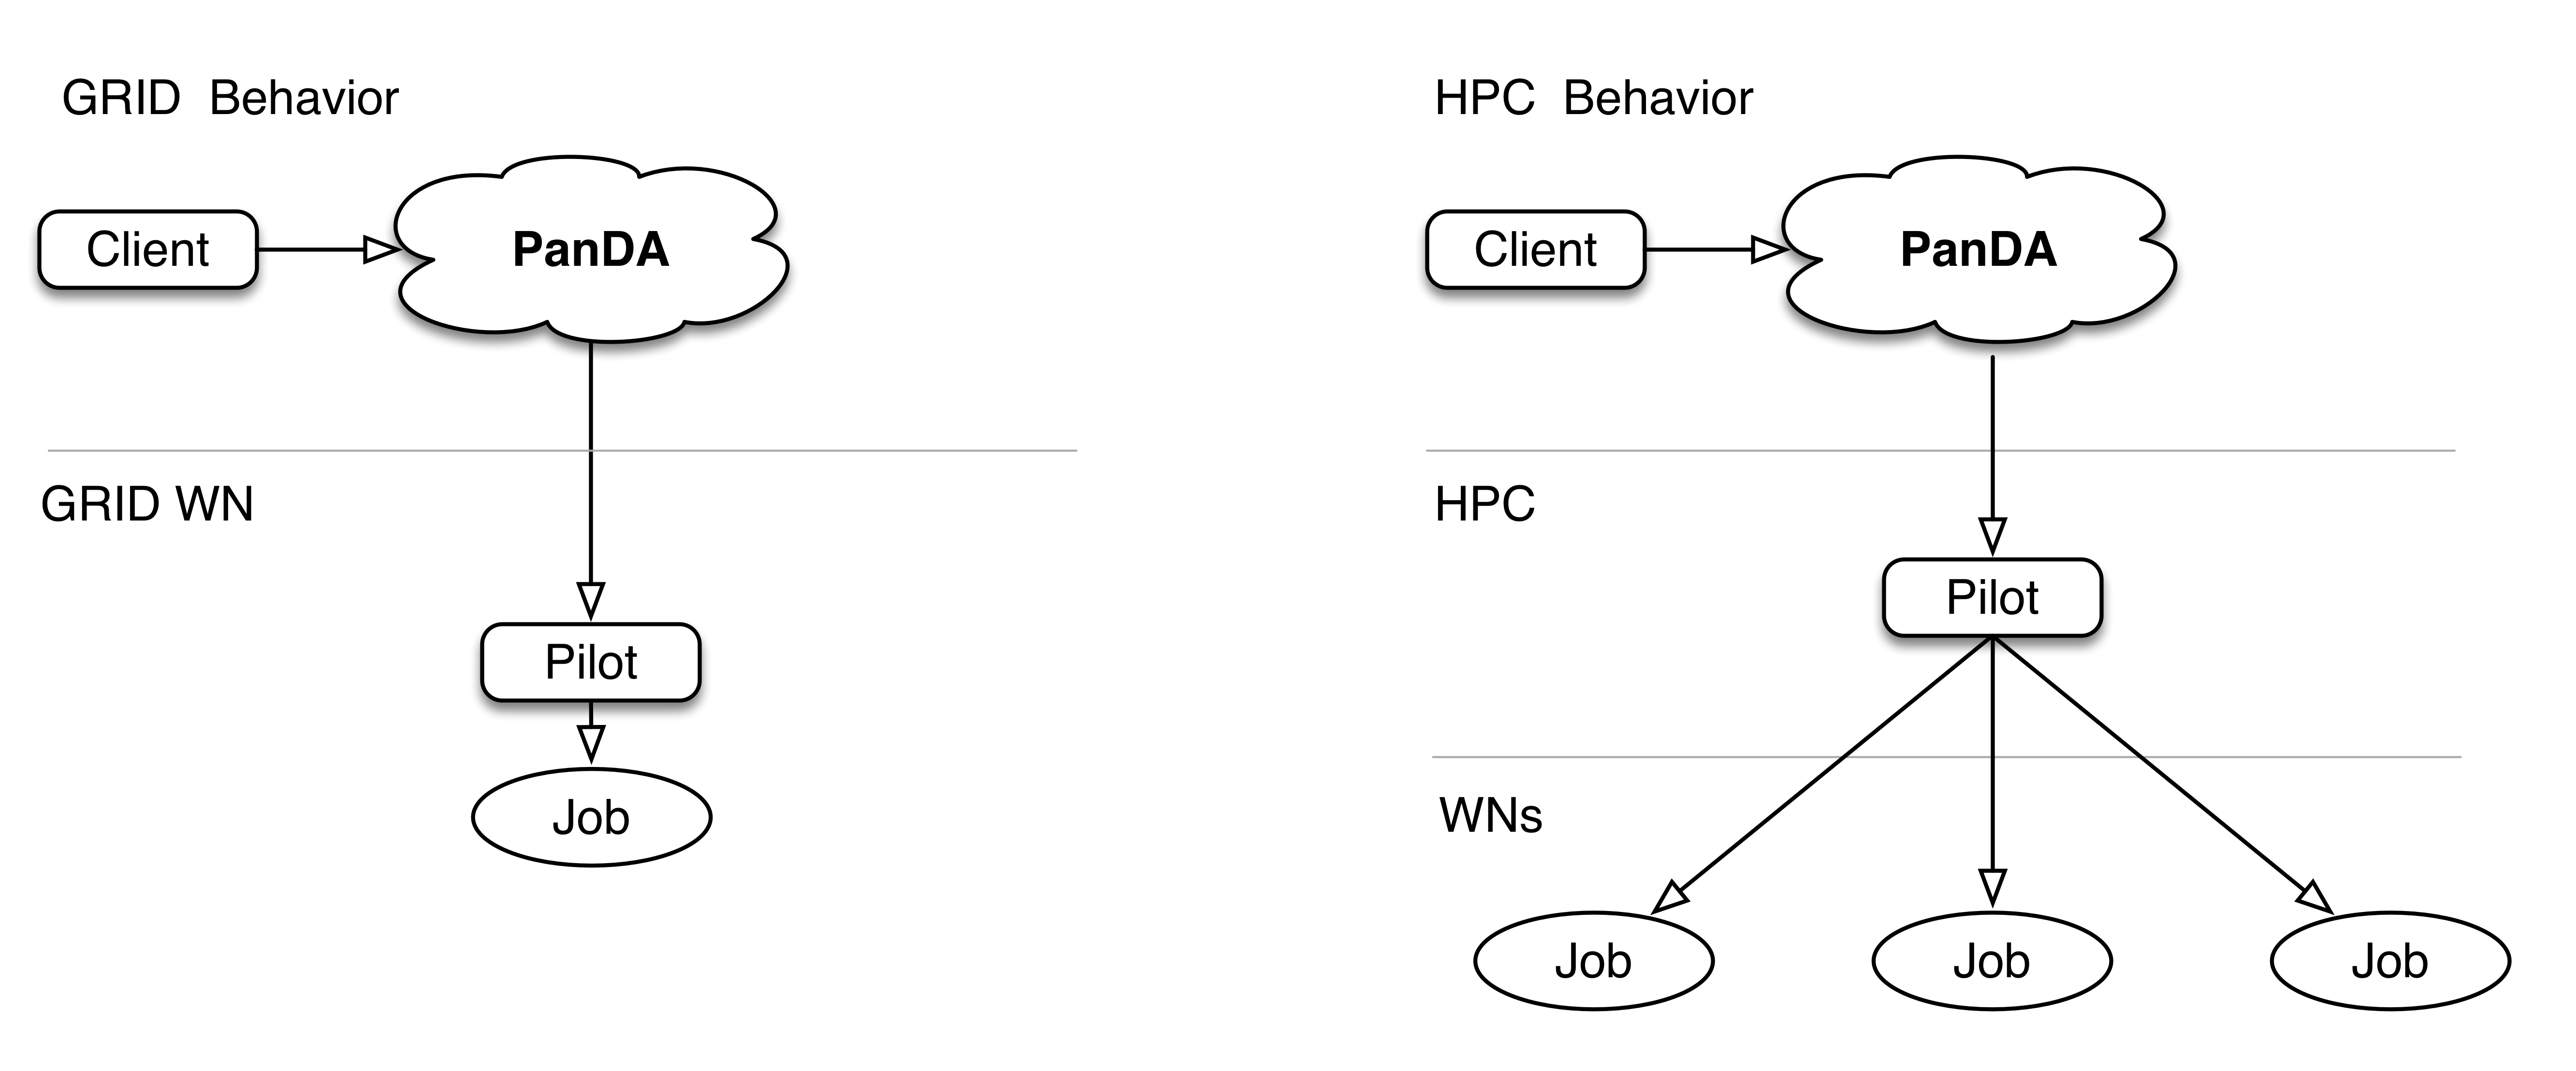
\includegraphics[width=0.75\textwidth]{images/Figure_3.png}
% figure caption is below the figure
%\caption{A concept for the launching of multiple PanDA jobs on HPC with the
%limited number of Job Slots in comparison with regular GRID launch}
%\label{fig:launching}
%\end{figure*}

% For two-column wide figures use
%\begin{figure*}
% Use the relevant command to insert your figure file.
% For example, with the graphicx package use
%  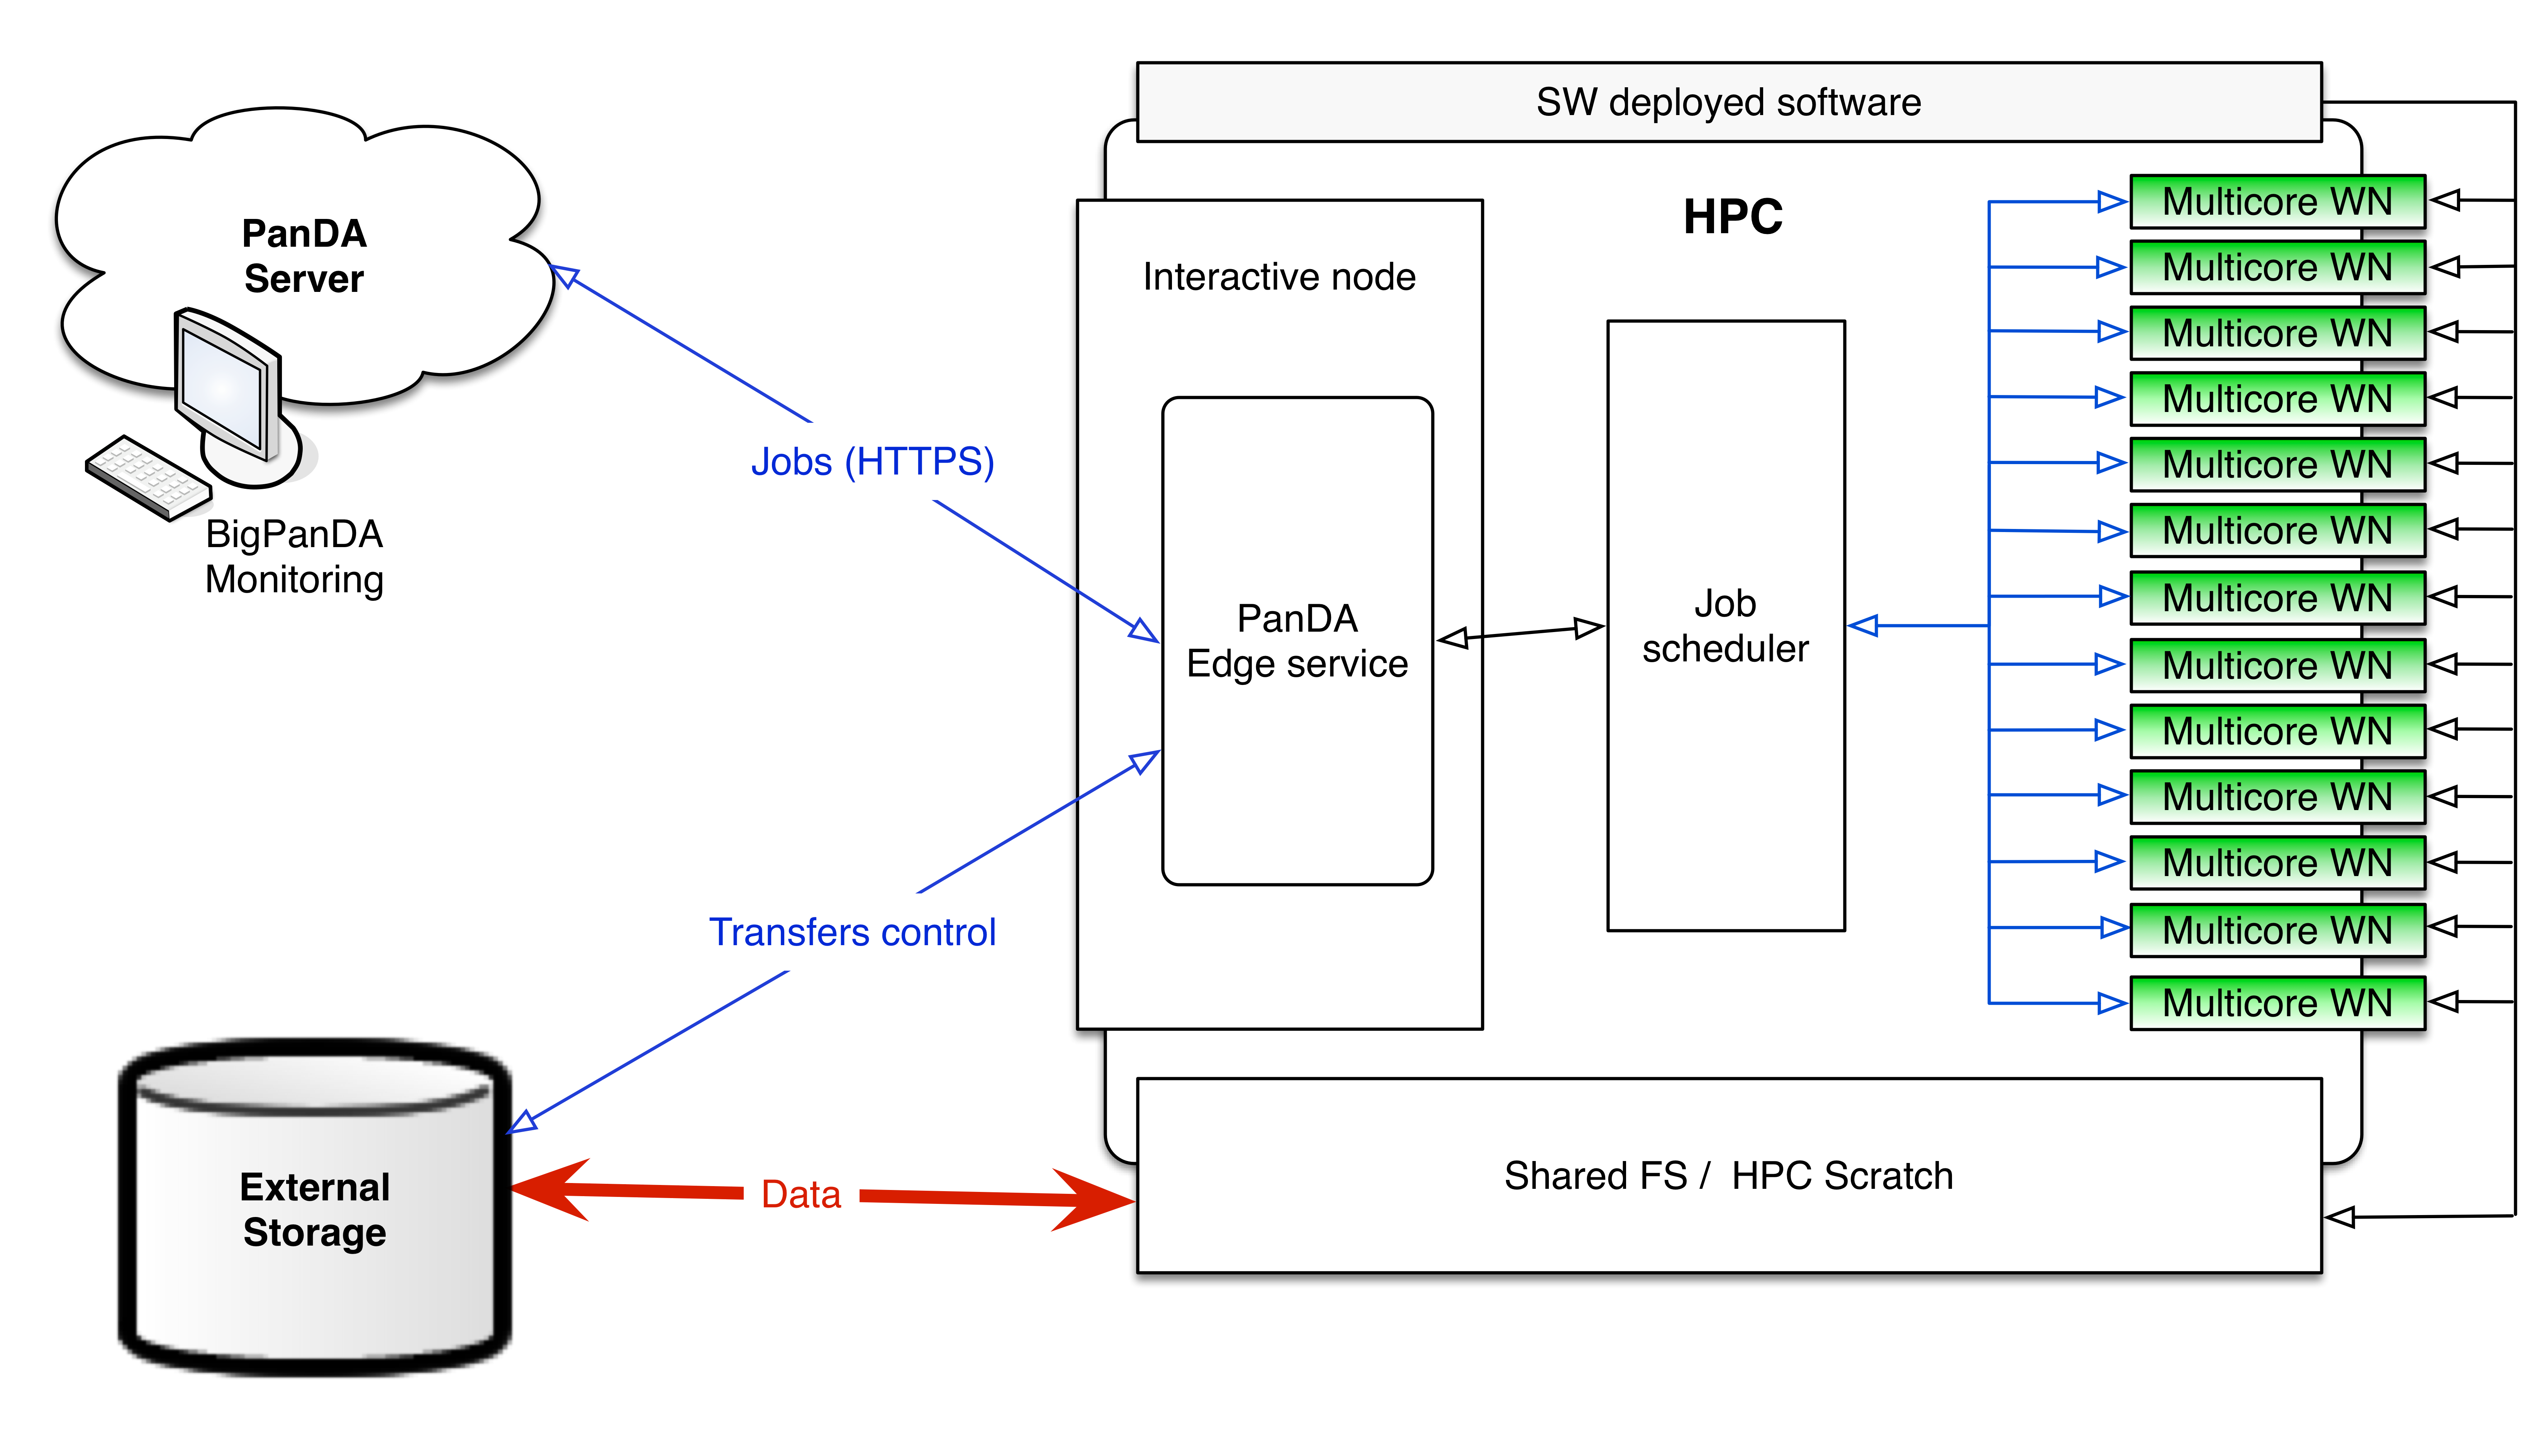
\includegraphics[width=0.75\textwidth]{images/Figure_4.png}
% figure caption is below the figure
%\caption{A concept of integration of LCF(HPC) with PanDA}
%\label{fig:integration}
%\end{figure*}

% For two-column wide figures use
\begin{figure*}
% Use the relevant command to insert your figure file.
% For example, with the graphicx package use
  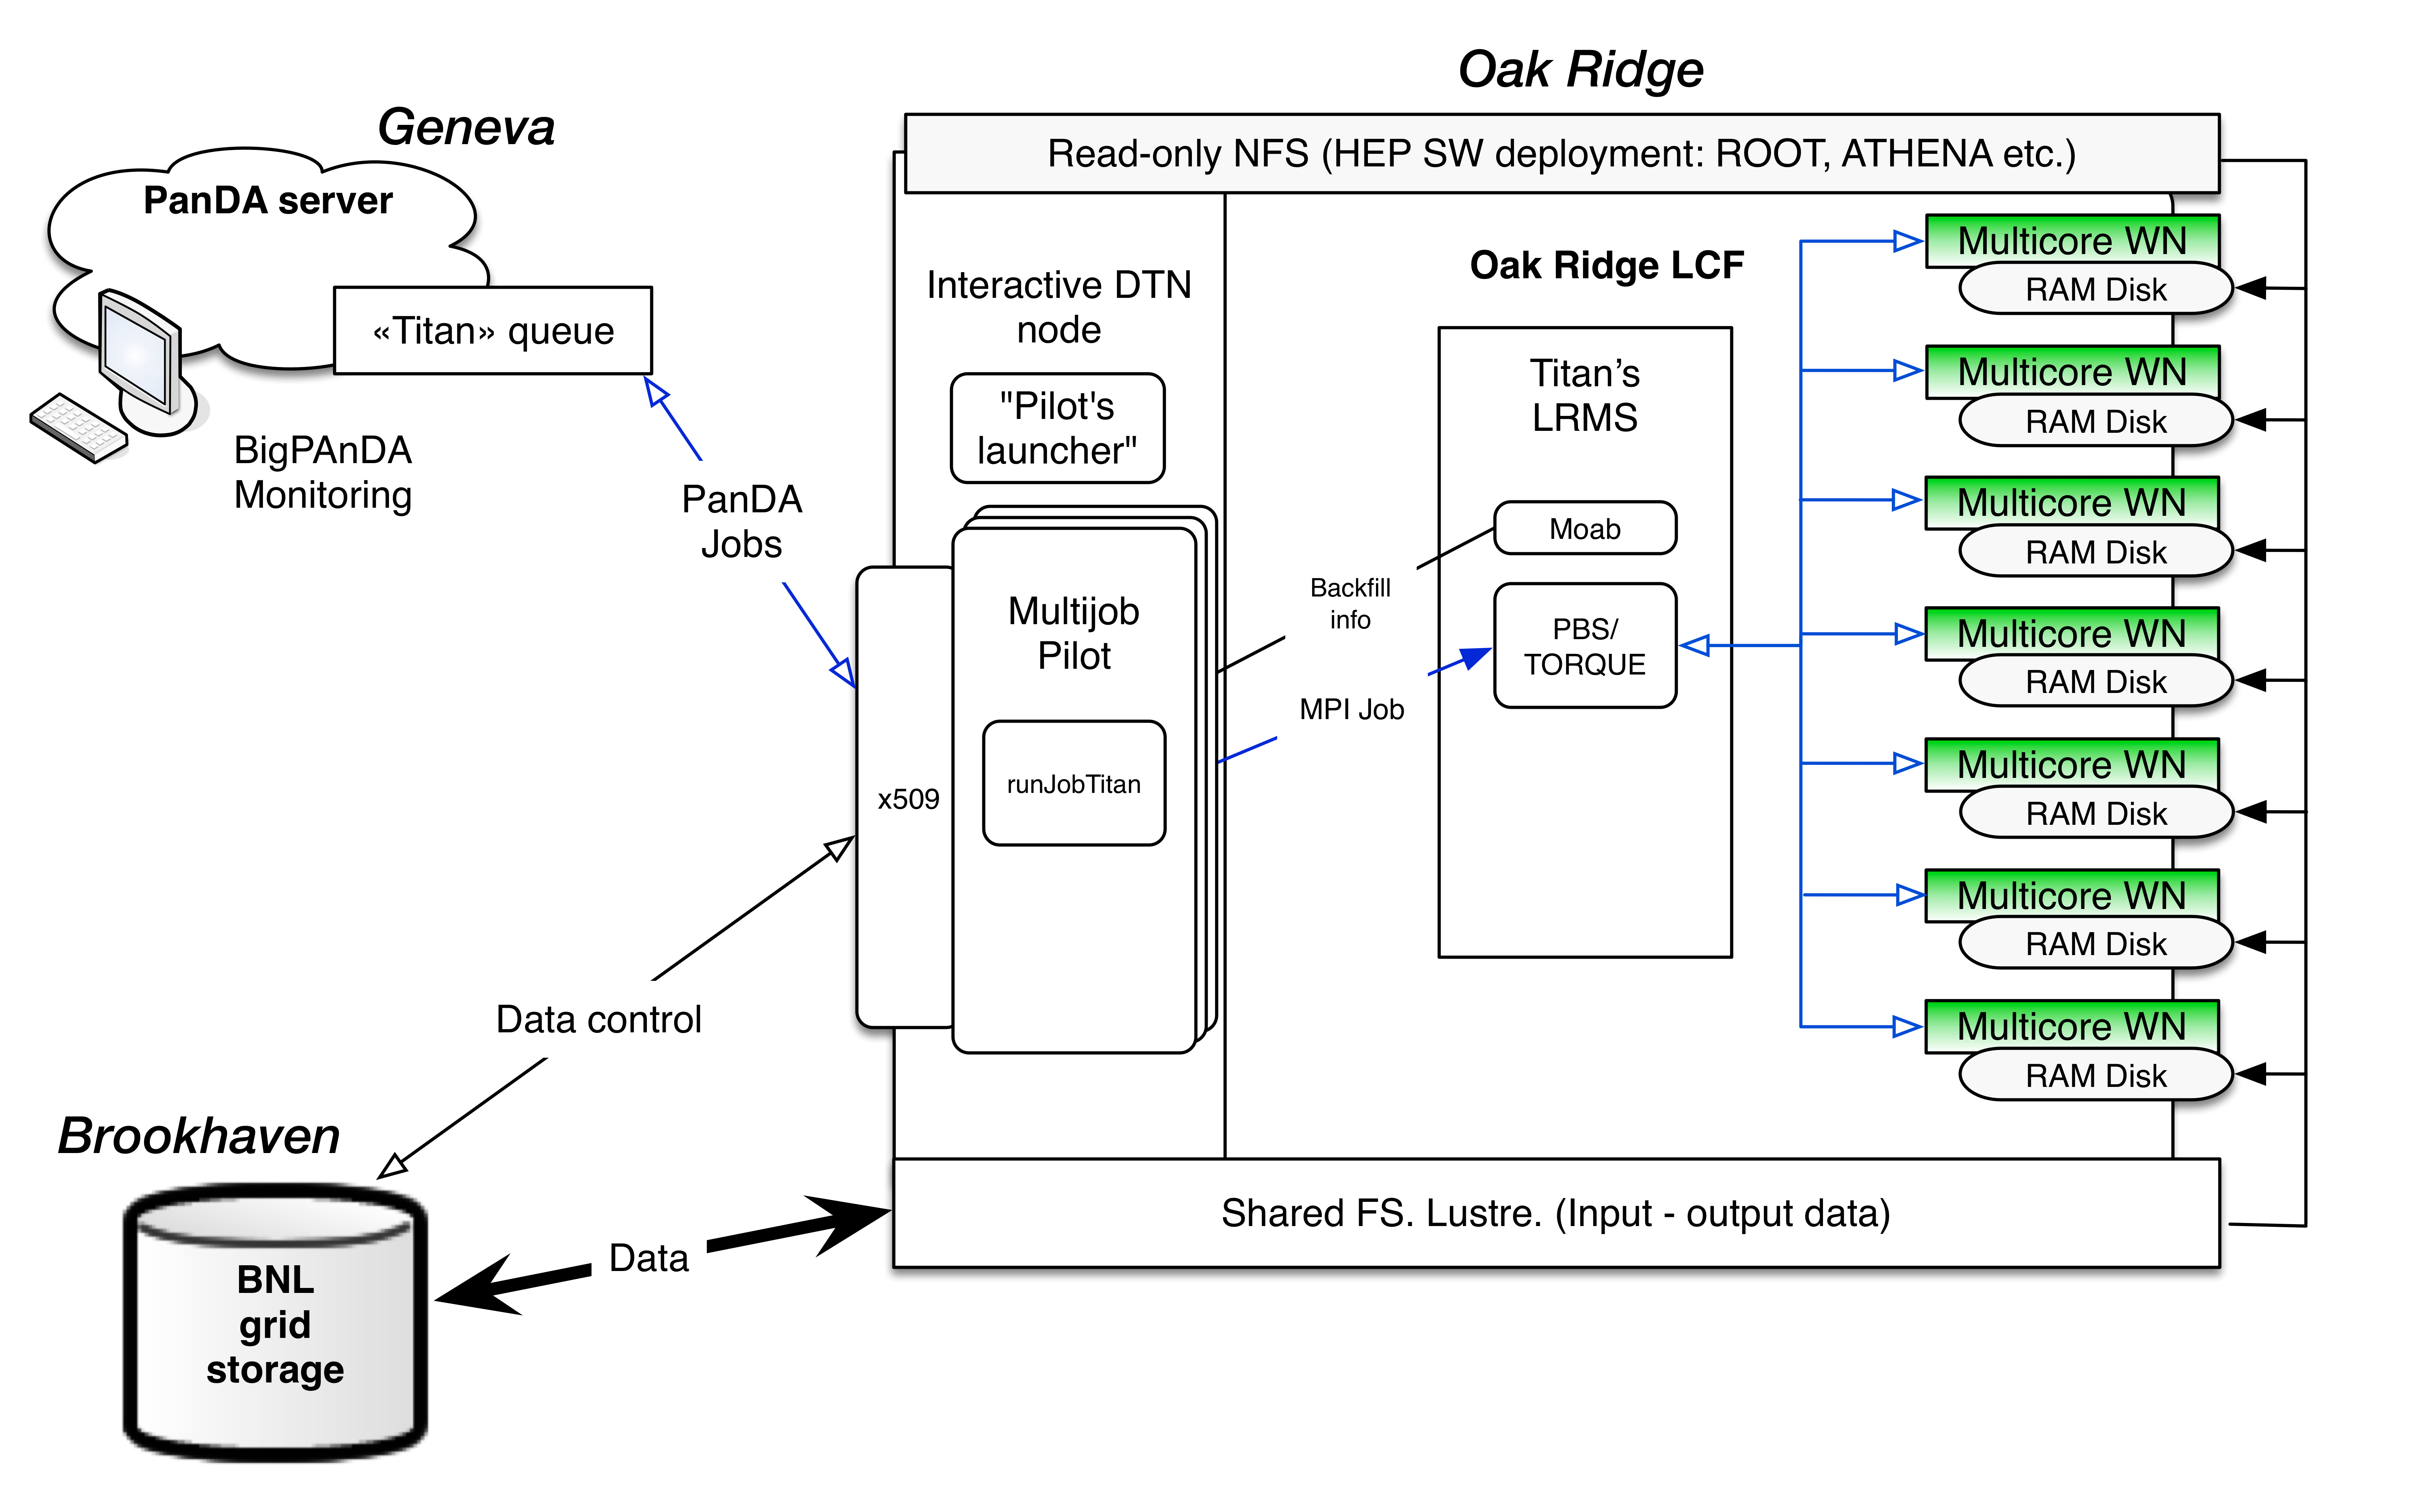
\includegraphics[width=0.75\textwidth]{images/Figure_5.png}
% figure caption is below the figure
\caption{Schematic view of PanDA WMS integration with Titan supercomputer at OLCF}
\label{fig:implementation}
\end{figure*}


% For two-column wide figures use
\begin{figure*}
% Use the relevant command to insert your figure file.
% For example, with the graphicx package use
  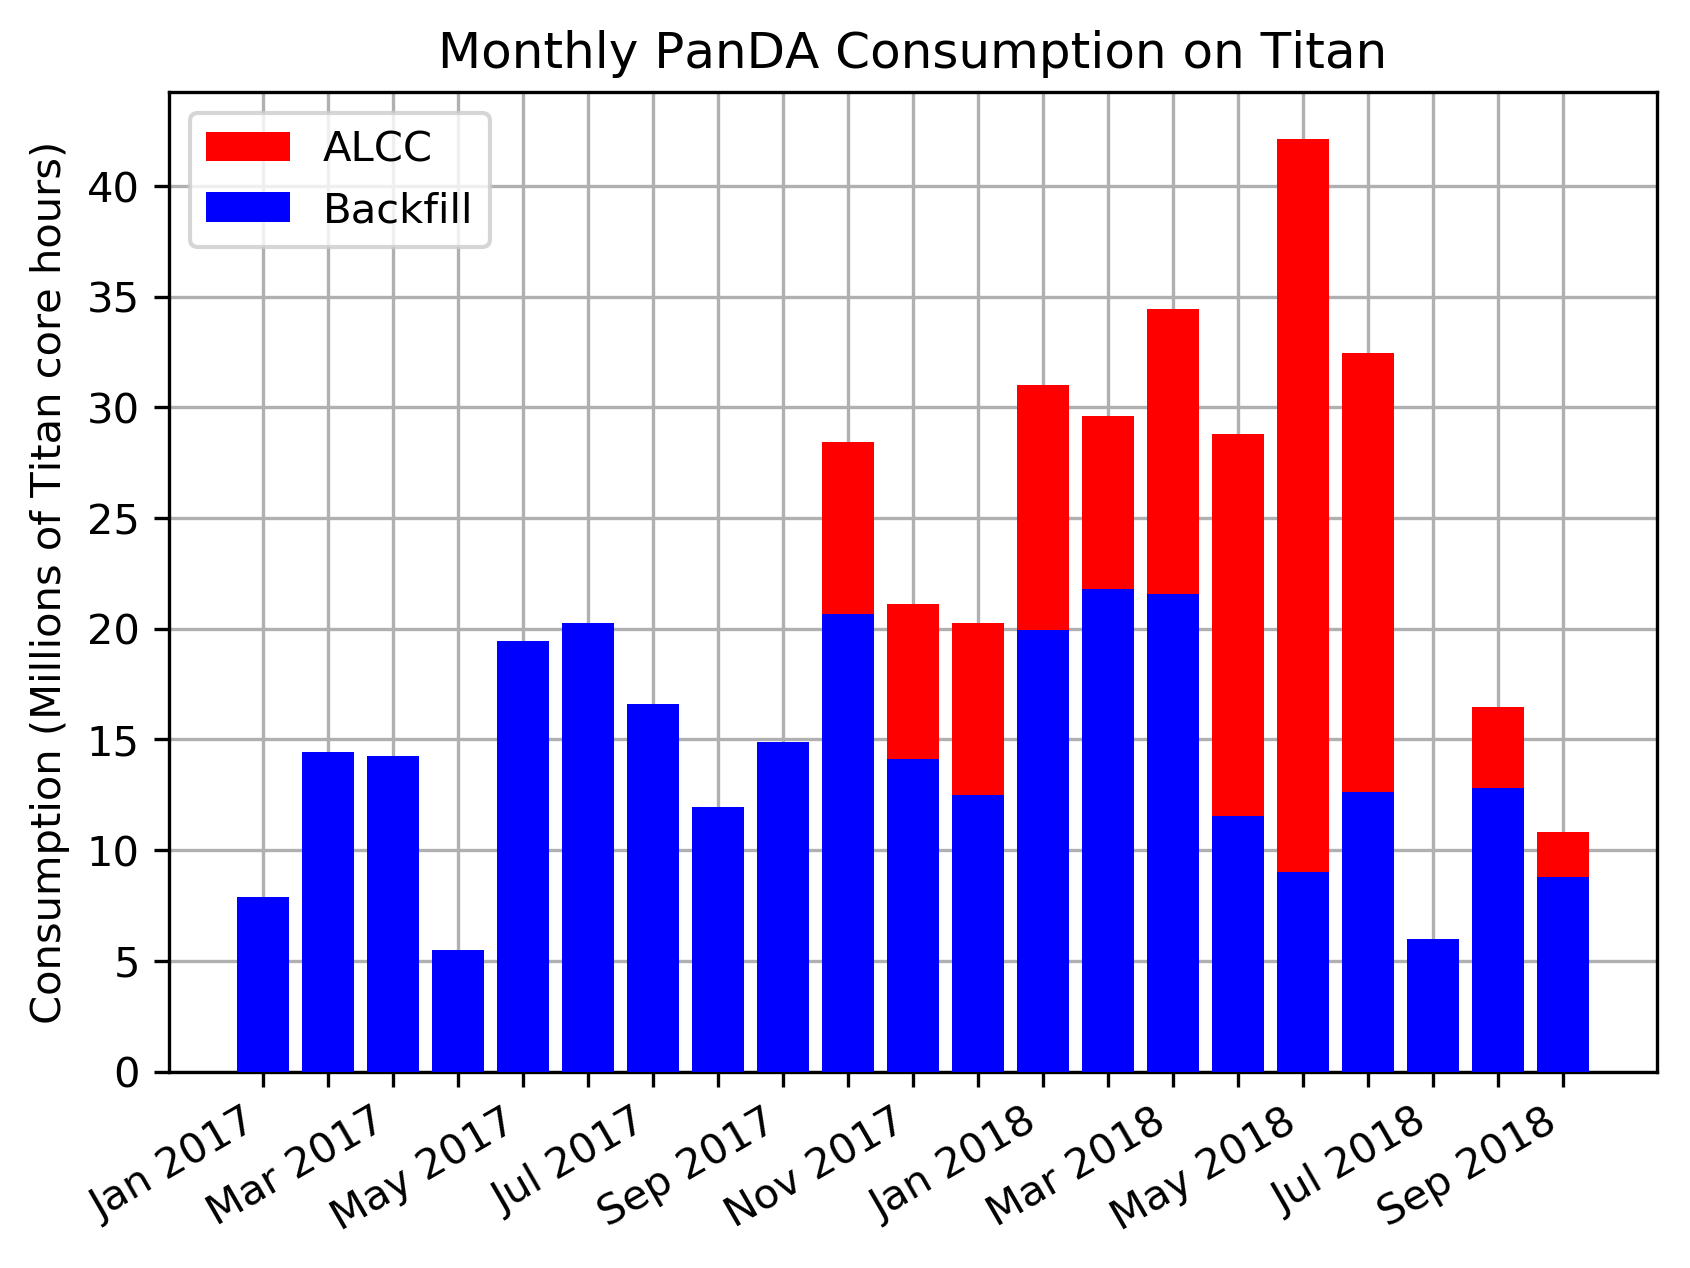
\includegraphics[width=0.75\textwidth]{images/monthly-consumption.png}
% figure caption is below the figure
\caption{This figure shows the monthly consumption of resources on Titan by the
two methods used by PanDA.}
\label{fig:monthly-consumption}
\end{figure*}


%-  vim:set syntax=tex:
